\documentclass[12pt, a4paper]{article}
\usepackage[left=2.5cm, right=2.5cm, top=2cm]{geometry} 
\usepackage{graphicx}
\usepackage{tabularx}

%\documentclass[a4paper,10pt]{scrartcl}

\usepackage[utf8]{inputenc}

\title{Programa de Aula: Samba de Gafieira - Nível I}
\author{Fernando Pujaico Rivera}
\date{}

\pdfinfo{%
  /Title    (Sílabus: Samba de Gafieira - Nível I )
  /Author   (Fernando Pujaico Rivera)
  /Creator  ()
  /Producer ()
  /Subject  ()
  /Keywords (Samba, Gafieira)
}


\begin{document}
{\let\newpage\relax\maketitle}
A Tabela \ref{tab:typospos} e \ref {tab:typosmov}, descrevem a notação de nomes  (posturas e movimentos) usadas 
na descrição do programa de aula.
A Figura \ref{fig:mov} mostra como são relacionados as posturas e os distintos tipos de movimentos.


\begin{table}[h]
\centering
\begin{tabular}{|p{3cm}|p{13cm}|}
\hline
~ & Descrição \\  \hline
Postura & No transcurso das aulas, chamaremos postura o pose, a una distribuição estática
dos membros do corpo. Uma postura estabelece um ponto de inicio para a execução de um
movimento; assim, um movimento inicia e termina sempre numa postura o pose.\\ \hline

\end{tabular}
\caption{Descrição de uma postura}
\label{tab:typospos}
\end{table}


\begin{table}[h]
\centering
\begin{tabular}{|p{2.5cm}|p{13.5cm}|}
\hline
~ & Descrição \\  \hline
\textbf{Movimento} & É chamado como movimento ou ação, a um conjunto de trocas de peso ou deslocamentos de membros.
Um movimento não necessariamente tem um nome próprio, se tiver, neste documento este será
chamado como passo.\\ \hline
\textbf{Transição ou movimento de transição} &  Movimento extremadamente simples, pelo qual geralmente não tem nome próprio,
e constam de poucas trocas de peso e deslocamentos de membros. Exemplo: transição entre Frente trás e o Balanço, 
ou a transição entre Balanço e o Cruzado. Algumas transições
pelo seu uso na samba de gafieira, tem ganhado um nome próprio, estes são: Saída lateral e Gancho.\\ \hline
\textbf{Passo (básico)} & Movimento de nível iniciante; o conhecimento deste tipo de
movimentos é necessário para enlaçar/interconectar movimentos mais complexos ensinados nas aulas. Estes
movimentos tem uma característica cíclica, é dizer, a postura do final do movimento 
é igual à postura de inicio. Os passos básicos são: Frente e trás (F.T.), Balanço e Cruzado.\\ \hline
\textbf{Passo} &  Movimento genérico com uma amplitude de dificuldade desde simples ate complexo.
Um passo inicia e termina numa postura, a qual pode ser a mesma. Definiremos como passo, a um movimento
notável, de modo que este tem ganhado um nome próprio; exemplo: Gatilho, Gancho redondo, Romário, Puladinho, Elástico, etc. \\ \hline
\end{tabular}
\caption{Tipos de movimentos.}
\label{tab:typosmov}
\end{table}


\begin{figure}[h]
  \centering
  \caption{ Movimento sendo executado desde uma postura ate outra postura.}
  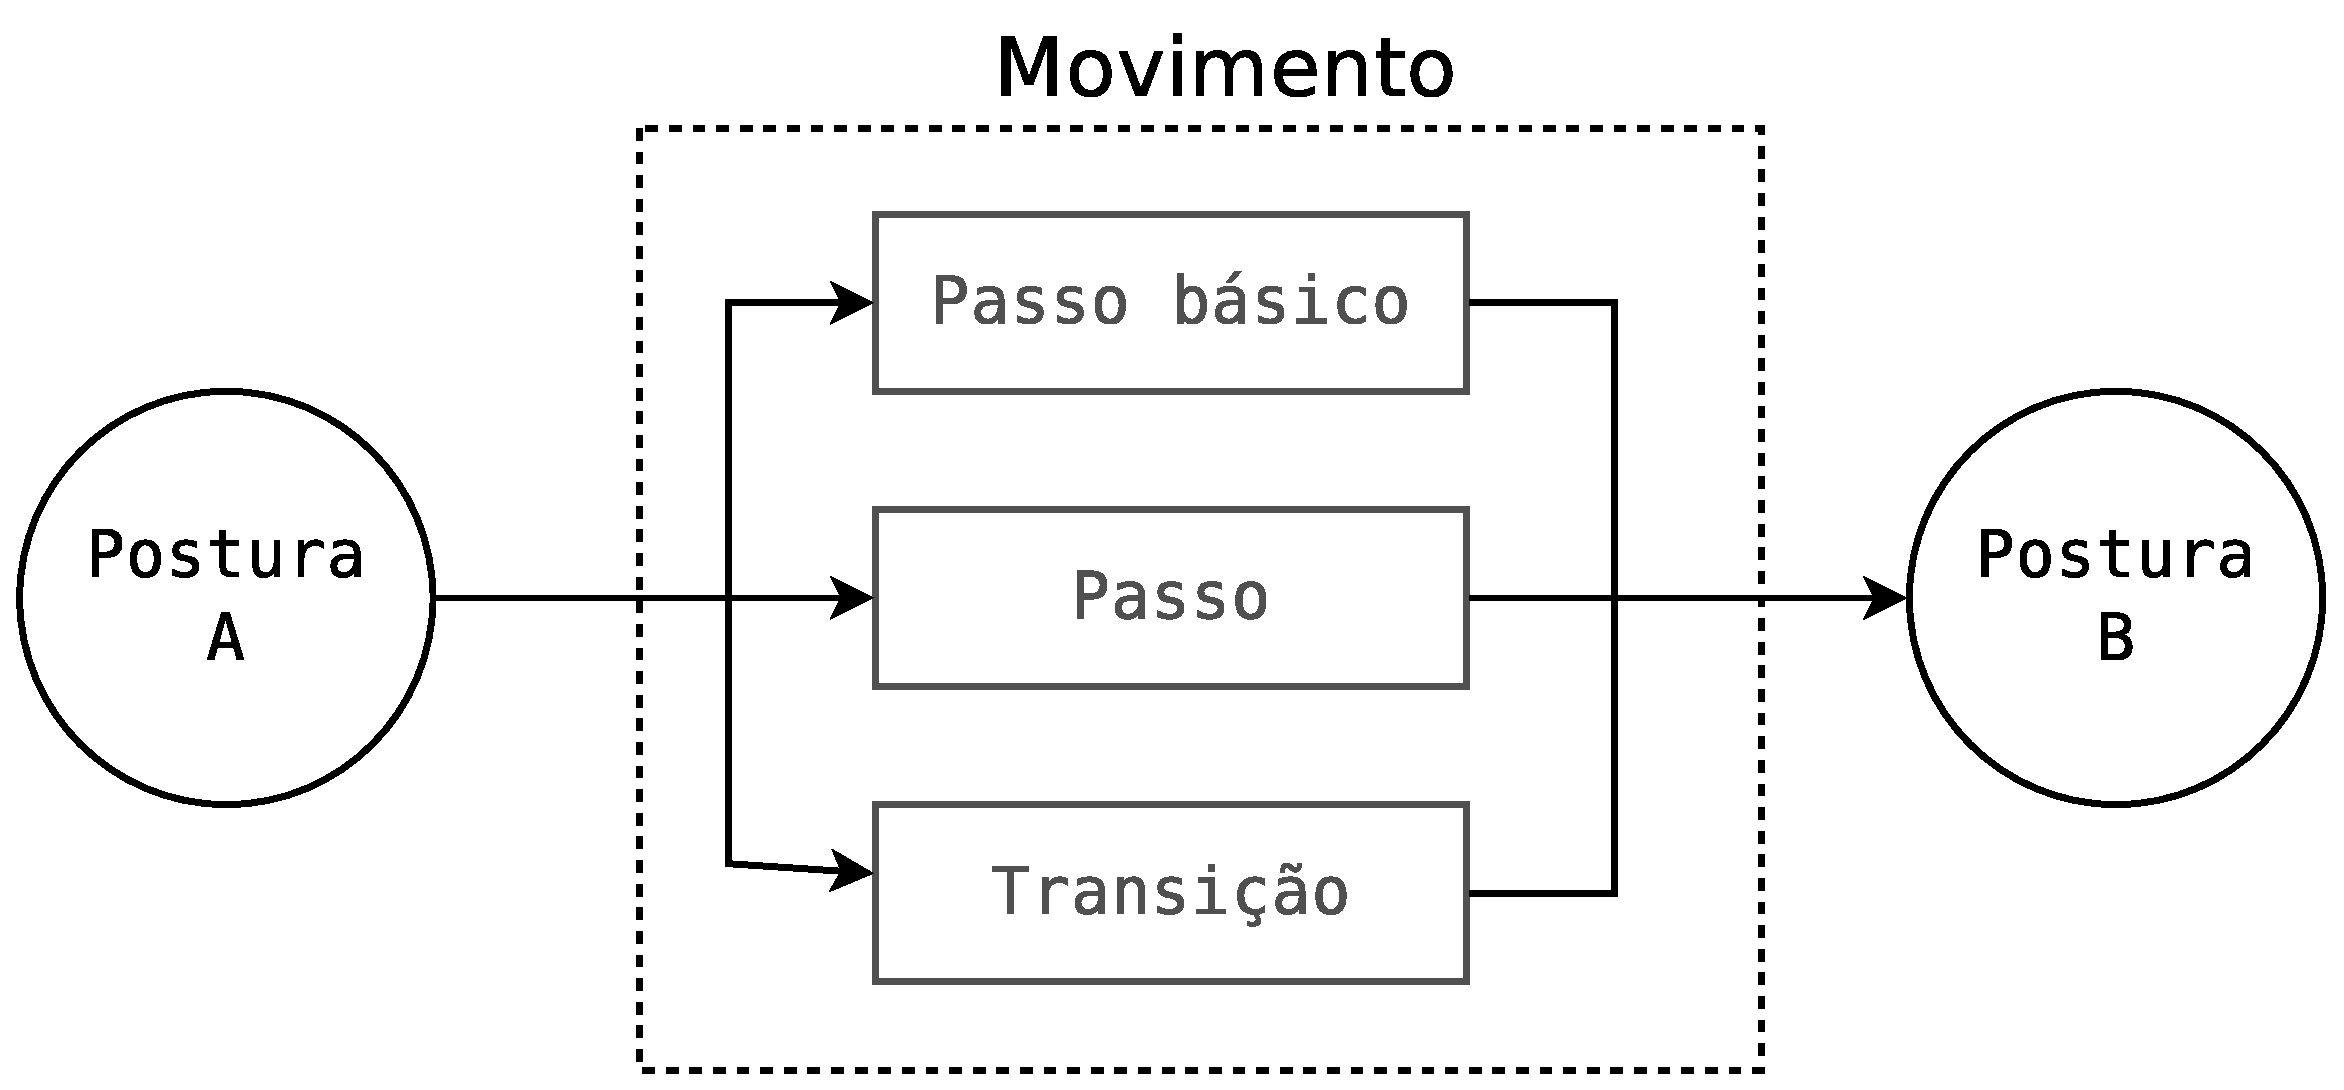
\includegraphics[width=0.7\textwidth]{Diagrama1.eps}% picture filename
  \label{fig:mov}
\end{figure}





As Tabelas \ref{tab:myfirsttable},\ref{tab:myfirsttable2} e \ref{tab:myfirsttable3} 
mostram a descrição do conteúdo das aulas de samba de gafieira.

%%%%%%%%%%%%%%%%%%%%%%%%%%%%%%%%%%%%%%%%%%%%%%%%%%%%%%%%%%%%%%%%%%%%%%%%%%%%%%%%
%%%%%%%%%%%%%%%%%%%%%%%%%%%%%%%%%%%%%%%%%%%%%%%%%%%%%%%%%%%%%%%%%%%%%%%%%%%%%%%%
\begin{table}[h]
\centering
\begin{tabular}{|p{0.5cm}|p{3.0cm}|p{12.0cm}|}
\hline
S. & Tema & Descrição \\  \hline \hline
1 &  \textbf{Passos básicos:} Frente e trás (F.T.) e Balanço & Serão estudados os movimentos de transição entre o balaço e o F.T.. 
        \begin{itemize}
        \item Explicação dos termos: compasso binário, tempo forte e fraco, frase musical + frase com final conclusivo/suspensivo.
        \item Boas praticas no abraço para a dança (Braços do condutor). 
        \item Descrição temporal dos movimentos (em termos de rápido e lento).
        \end{itemize}
        \\ \hline
2 &  \textbf{Passo básico:} Cruzado &  Serão estudados os movimentos de transição entre o balaço e o cruzado, além de enfeites no cruzado. 
        \begin{itemize}
        \item Repasso: F.T. (tango vs samba - pés juntos e cadencia) e balanço + giro. 
        \item Abraço na dança (Braços do seguidor).
        \item Treinamento do passo básico em frases com terminação conclusiva. 
        \item Explicação dos termos: legato e staccato.
        \item Descrição rítmica dos movimentos (em termos de médio tempo e tempo).
        \end{itemize}
        \\ \hline
3 &  \textbf{Transição:} Saída lateral. &  Serão estudados os movimentos de transição entre F.T. e cruzado e enfeites na saída lateral. 
        \begin{itemize}
        \item Treinamento de olhos vendados (condutor) + balanço/F.T. Descobrir pé de apoio do seguidor.
        \item Treinamento do passo básico em frases com terminação suspensiva. 
        \item Explicação dos termos: condução, indução, coreografia, condução compartilhada.
        \item Consciência corporal: passando 1 bolinha no casal para isolar a parte superior e inferior do corpo.
        \end{itemize}
        \\ \hline
4 &  \textbf{Transição:} gancho. \textbf{Postura:} X &  Serão estudados os movimentos de transição entre cruzado e F.T., além das posturas notáveis.
        \begin{itemize}
        \item Treinar mudando entre F.T., deslocando e no lugar, com a mudança da frase musical.
        \item Treinamento de  olhos vendados (seguidor) + terminação conclusiva.
        \item Treinamento sobre indução (só caminhar).
        \item Consciência corporal: jogando 1 bolinha no casal para isolar a parte superior e inferior do corpo.
        \end{itemize}
        \\ \hline 
\end{tabular}
\caption{Descrição do conteúdo do mês 1}
\label{tab:myfirsttable}
\end{table}

%%%%%%%%%%%%%%%%%%%%%%%%%%%%%%%%%%%%%%%%%%%%%%%%%%%%%%%%%%%%%%%%%%%%%%%%%%%%%%%%
%%%%%%%%%%%%%%%%%%%%%%%%%%%%%%%%%%%%%%%%%%%%%%%%%%%%%%%%%%%%%%%%%%%%%%%%%%%%%%%%
\begin{table}[h]
\centering
\begin{tabular}{|p{0.5cm}|p{3.0cm}|p{12.0cm}|}
\hline
S. & Tema & Descrição \\  \hline \hline            
5 &  \textbf{Passo:} Gatilho &  Será estudado a distribuição de tempos e movimentos do passo gatilho.
        \begin{itemize}
        \item Repasso: Gancho e cruzado.
        \item Treinar girar o salão: usando balanço e F.T.
        \item Consciência corporal: balanço + passando 1 bolinha + pausas no final da frase musical.
        \end{itemize}
        \\ \hline 
6 &  \textbf{Passo:} Edmundo &  Será estudado o controle do equilíbrio e reconhecer eixo do corpo. 
        \begin{itemize}
        \item Treinar girar o salão: usando pisadas em tempo + pausas no final da frase musical.
        \item Treinamento sobre indução: sem musica, F.T com pausas do condutor.
        \item Consciência corporal: F.T. + passando 1 bolinha + pausas no final da frase musical.
        \end{itemize}
        \\ \hline 
7 &  \textbf{Passo:} Caminhada em contratempo & Será estudado a distribuição de tempos na caminhada em contratempo. 
        \begin{itemize}
        \item Isolamento de partes do corpo: passando uma bolinha no casal, em tempo, estando costa com costa.
        \item Treinamento sobre indução: sem musica, cruzado com pausas do condutor.
        \item Treinamento de pica-pau
        \item Treinamento da trança (individual).
        \end{itemize}
        \\ \hline 
8 &  \textbf{Passo:} Sacada de perna & Será estudado a sacada de perna (ambas pernas) terminando no cruzado. 
        \begin{itemize}
        \item Treinamento de olhos vendados (seguidor) + dançando.
        \item Treinamento sobre indução: cruzado com pausas no final da frase musical.
        \item Treinamento escovinhas para atrás.
        \item Treinamento de pica-pau (variantes)
        \end{itemize}
        \\ \hline 
\end{tabular}
\caption{Descrição do conteúdo do mês 2}
\label{tab:myfirsttable2}
\end{table}


%%%%%%%%%%%%%%%%%%%%%%%%%%%%%%%%%%%%%%%%%%%%%%%%%%%%%%%%%%%%%%%%%%%%%%%%%%%%%%%%
%%%%%%%%%%%%%%%%%%%%%%%%%%%%%%%%%%%%%%%%%%%%%%%%%%%%%%%%%%%%%%%%%%%%%%%%%%%%%%%%
\begin{table}[h]
\centering
\begin{tabular}{|p{0.5cm}|p{3.0cm}|p{12.0cm}|}
\hline
S. & Tema & Descrição \\  \hline \hline
9 &  \textbf{Passo:} Tesoura & Será estudado desde F.T. (balanço corre-corre) e outras opções de uso do passo.
        \begin{itemize}
        \item Treinar girar o salão: usando um passo triple em 2 tempos + pausas no final da frase musical.
        \item Treinamento escovinhas para a frente
        \item Consciência corporal: balanço + jogando 1 bolinha + pausas no final da frase musical.
        \end{itemize}
        \\ \hline 
10&  \textbf{Movimento:} escovinhas lateral desde X & Iniciaremos o estudo dos movimentos da família da Escovinha.
        \begin{itemize}
        \item Treinar girar o salão: dançando + pausas no final da frase musical.
        \item Consciência corporal: F.T. + jogando 1 bolinha + pausas no final da frase musical.
        \item Treinamento de pica-pau (variantes).
        \end{itemize}
        \\ \hline 
11&  \textbf{Movimento:} Sacada invertida com caminhada e escovinhas recuando & Estudaremos outra opção de Escovinha (opcionalmente se usa a Tesoura). 
        \begin{itemize}
        \item Treinamento de olhos vendados (seguidor) + dançando + pausas no final da frase musical.
        \item Treinamento escovinhas intercambiado lados (complexa).
        \item Definição de sincopa.
        \item Treinamento F.T. em frases com terminação em tempo fraco (sincopado).
        \end{itemize}
        \\ \hline 
12&  \textbf{Passo:} Assalto & Será estudado a diferença entre Assalto e Bailarina, adicionalmente serão agregados enfeites de mãos para o movimento. 
        \begin{itemize}
        \item Treinamento de olhos vendados (condutor) lembrar abraço,peso do corpo, pausas, etc.
        \item Treinamento dançando mudando de passo quando muda a frase musical.
        \item Treinamento escovinhas (para frente e atrás).
        \item Treinamento da trança (individual)
        \end{itemize}
        \\ \hline
\end{tabular}
\caption{Descrição do conteúdo do mês 3}
\label{tab:myfirsttable3}
\end{table}

%%%%%%%%%%%%%%%%%%%%%%%%%%%%%%%%%%%%%%%%%%%%%%%%%%%%%%%%%%%%%%%%%%%%%%%%%%%%%%%%
%%%%%%%%%%%%%%%%%%%%%%%%%%%%%%%%%%%%%%%%%%%%%%%%%%%%%%%%%%%%%%%%%%%%%%%%%%%%%%%%
\begin{table}[h]
\centering
\begin{tabular}{|p{0.5cm}|p{3.0cm}|p{12.0cm}|}
\hline
S. & Tema & Descrição \\  \hline \hline
13&  \textbf{Passo:} Romário & Será estudado a condução, postura do corpo e eixo para a execução do movimento, adicionalmente serão agregados dois enfeites para o movimento.
        \begin{itemize}
        \item Treinamento escovinhas intercambiado lados (complexa).
        \item Definição formal de motivo (usos), frase, período e sequencia.
        \item Longitudes mais prováveis da frase musical.
        \item Mickey mousing no cine e na dança.
        \end{itemize}
        \\ \hline
14&  \textbf{Passo:} Facão, \textbf{Postura}: Facão & Será estudado dois estilos de facão (movimento discreto e ondulado) e a postura de finalização. 
        \begin{itemize}
        \item Definição de leitmotif (leitmotiv) vs. tema, na musica.
        \item Definição de sublinhando (Underscoring) no cine, diferencias com o Mickey mousing.
        \end{itemize}
        \\ \hline
%15&  \textbf{Passo:} Puladinho & Será estudado a consciência corporal necessária para executar o movimento, adicionalmente será agregado um enfeite para o movimento. \\ \hline
\end{tabular}
\caption{Descrição do conteúdo do mês 4}
\label{tab:myfirsttable3}
\end{table}

\end{document}
